\begin{figure}[htb]
  \centering
  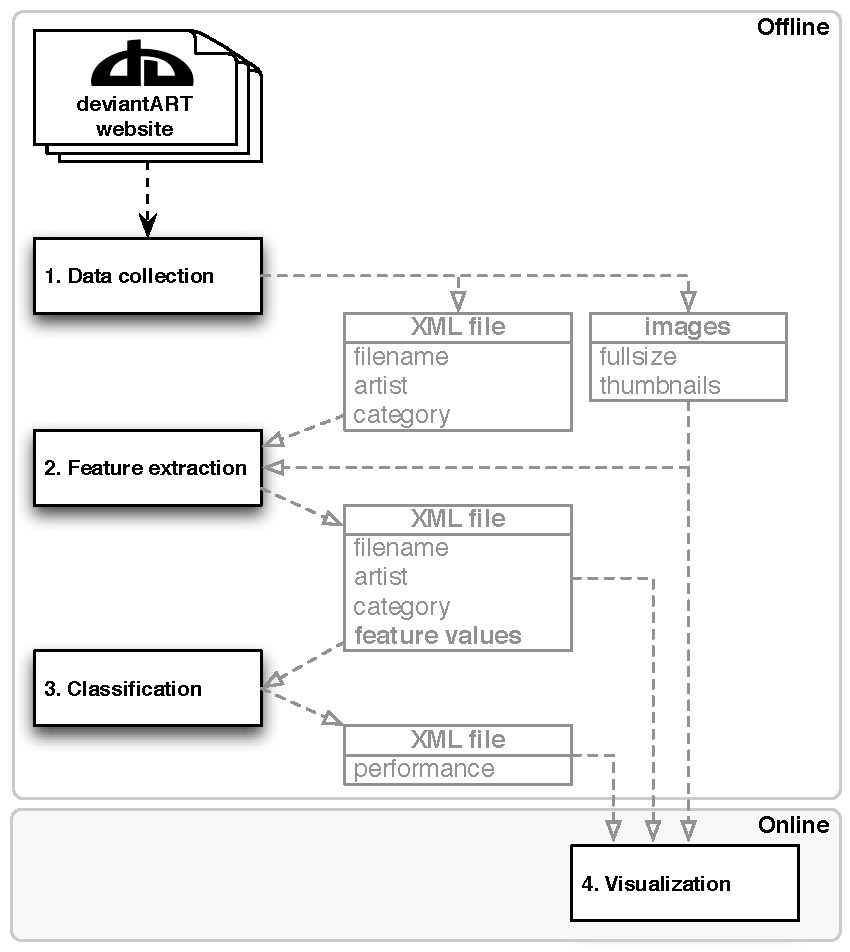
\includegraphics[width=1\linewidth]{img/components.pdf}
  \caption{Interaction between the four components of the toolkit.}
  \label{fig:components}
\end{figure}

The toolkit consists out of four replaceable components with varying degrees of integration.
Each component writes its output (e.g. image information and features) to a XML file.
The first three components are all executed \textit{offline} (precomputed), while the visualization component allows \textit{online} interaction with the images, features and classification results.
Figure~\ref{fig:components} provides an overview of all components and the data flow between them.

% toolboxes used
\subsection{Data collection}
The data collection component deals with downloading information and galleries from the dA website and it can easily be replaced to deal with different art communities.
% to allow the toolkit to be flexible and to be able

dA does not provide a web API to download images and therefore the backend links of the galleries to the RSS XML files were followed to access the image data.
For each image general information such as category, deviantART link and filename are stored, and the full image and 
thumbnails are downloaded.

For the network information collection, the friends pages of the users are parsed. No RSS XML files are provided by deviantART for this information, instead the HTML pages were parsed.


\subsection{Feature extraction}
The features implemented are show in Table \ref{tab:featurelist}.
All toolkits and libraries used in this research field, as well as the code to extract the features, are interfaced through the Matlab programming language.
Part of the statistical feature calculations were performed using openCV\footnote{http://opencv.willowgarage.com}~\cite{openCV} to speed up the feature extraction. openCV was used for color-space transformations, edge, corner and face-detection.

As explained in section~\ref{proposed-cognitive}, the toolkit includes cognitive-inspired features. First a saliency map and 4 conspicuity maps (color, intensity, orientation and skin) are computed and then the features are extracted. To create those maps Itti's model \cite{Itti_model} has been used because of its low computational time and the existence of a free toolkit \footnote{\url{http://www.saliencytoolbox.net}}. 

The XML-processing was done using an open-source XML-toolkit\footnote{\url{http://www.mathworks.com/matlabcentral/fileexchange/4278}}.

\begin{table}[htb]
    \centering
    \begin{tabular}	{ | l | l | } 
		\hline
		Feature name & type \\
		\hline
<<<<<<< .mine
		RGB & mean, median \\
		RGB compositional & mean, median \\
		HSV & mean, median \\
		HSV compositional & mean, median \\
		Intensity & mean, median, variance, entropy \\
		Intensity compositional & mean, median \\				
		Edges & edge to pixel ratio \\
		Edges compositional & edge to pixel ratio \\
		Corners & corner to pixel ratio \\
		Corners compositional & corner to pixel ratio \\
		Face detection & number of faces \\
		Saliency map & std. deviation, entropy, 3 most salient points  \\
		Conspicuity maps & std. deviation, entropy, skin ratio \\		
=======
		RGB & mean, median \\
		RGB compositional & mean, median \\
		HSV & mean, median \\
		HSV compositional & mean, median \\
		Intensity & mean, median, variance, entropy \\
		Intensity compositional & mean, median \\				
		Edges & edge to pixel ratio \\
		Edges compositional & edge to pixel ratio \\
		Corners & corner to pixel ratio \\
		Corners compositional & corner to pixel ratio \\
		Face detection & number of faces \\
		Saliency map & std. deviation, entropy, \\
		& 3 most salient points  \\
		Conspicuity maps & entropy, skin ratio \\		
>>>>>>> .r663
		\hline
    \end{tabular}
    \caption{Overview of implemented features}
    \label{tab:featurelist}
\end{table}

\subsection{Classification}
The classification component of the toolkit is implemented in Matlab.
For kNN, Naive Bayes, Nearest Mean classifiers and feature selection, PRTools\footnote{http://prtools.org} \cite{Duin00prtoolsversion} was used.
The PRTools toolkit provides functions to create a dataset format that can be used for all the used classifiers.
%Furthermore, the dataset can be managed using this toolkit.

LibSVM\footnote{\url{http://www.csie.ntu.edu.tw/~cjlin/libsvm/}} \cite{chang2001libsvm} for Matlab was used as SVM classifier because its high processing speed.


\subsection{Visualization}
The final component of the toolkit is the visualization application.
It is used to present the information that has been gathered by the other components.
The collected images are used together with the extracted image features (Figure~\ref{fig:components}) to visualize the dataset.
This provides an effective way to find patterns in the dataset, analyze classification results and filter information.
The application combines three different visualization techniques into one application, each of them offering a different look on the dataset.

The application is written in the Java programming language.
The open source Processing API\footnote{\url{http://www.processing.org}} is used to draw the visualizations.
The Processing API contains classes and functions that simplify drawing, animations and interactions in Java.
Processing was an obvious choice, because it has the right combination of cost, ease of use and speed~\cite{fry08}.

\begin{figure}[htb]
  \centering
  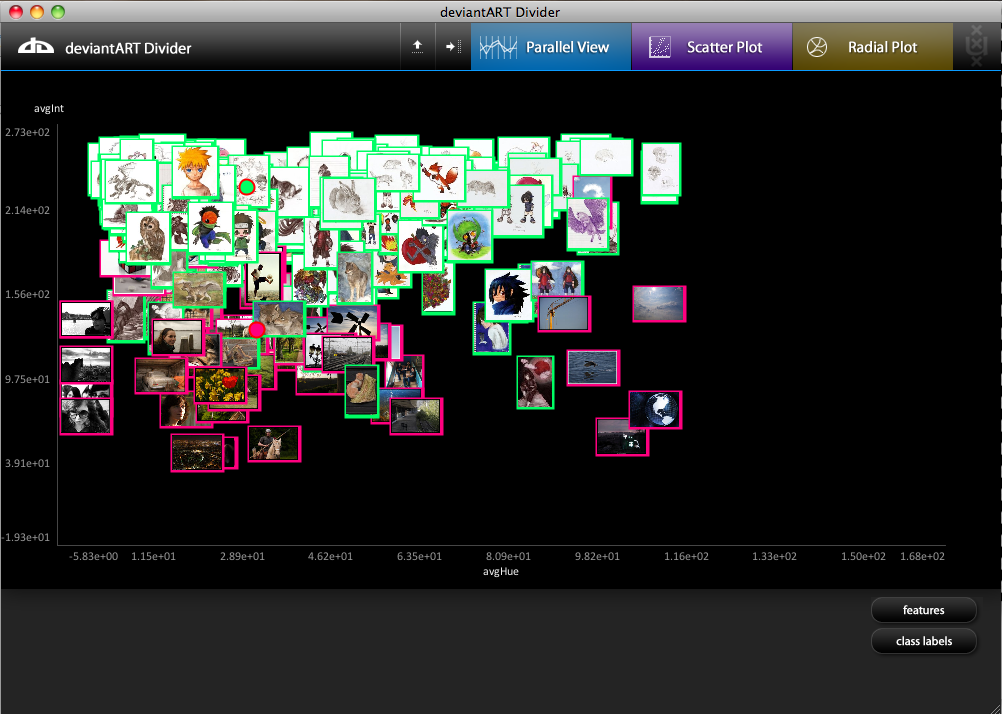
\includegraphics[width=1\linewidth]{img/visualization_scatter.png}
  \caption{The visualization application displaying a scatter plot of 2 artists, using average intensity and average hue as dimensions.}
  \label{fig:visualization_scatter}
\end{figure}

Figure~\ref{fig:visualization_scatter} shows the \textit{scatter plot} visualization technique.
The scatter plot displays values for two variables, which are image features that has been computed by the feature extraction component.
The data is displayed as a collection of thumbnail images.
Each thumbnail has the value of one feature determining the position on the horizontal axis and the value of the other feature determining the position on the vertical axis.
The border around each image represents the class (artists or categories) to which an image belongs.
For example, the images with a green border belong to the artist \textit{Kitsunebaka91} and the images with a red pink border belong to the artist \textit{Woekan}.
The user has full control over which classes are displayed in the visualization.
The users can also control which two features are used as variables on the horizontal and vertical axis of the scatter plot.
A single image or all the images belonging to one class can be highlighted, making it easier to recognize patterns.
The full version of a miniature image can be displayed to inspect it in more detail.

\begin{figure}[htb]
  \centering
  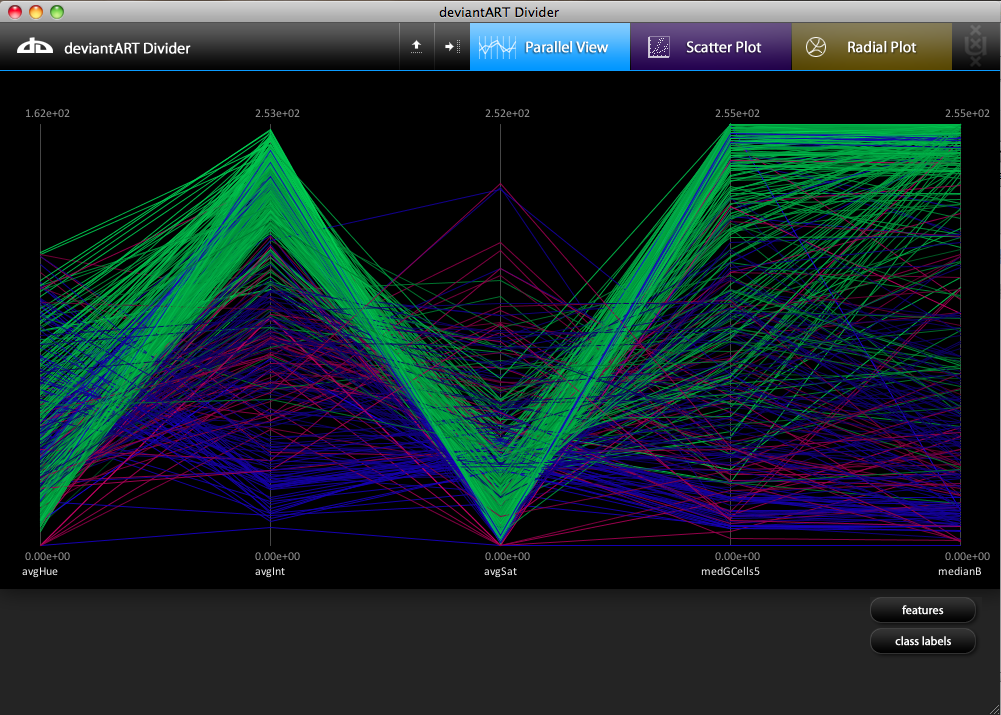
\includegraphics[width=1\linewidth]{img/visualization_parallel.png}
  \caption{The visualization application displaying a parallel coordinates plot of 3 artists and 5 features.}
  \label{fig:visualization_parallel}
\end{figure}

The scatter plot is limited to displaying only two features at the same time.
Figure~\ref{fig:visualization_parallel} shows the \textit{parallel coordinates} visualization technique~\cite{andrienko2001constructing}, a common way of visualizing high-dimensional data.
This enabled users to visualize beyond two features at the same time.
The two axes of the scatter plot are now replaced by $n$ vertical parallel lines to represent $n$ features ($n$-dimensional space).
An image is represented as a polyline with vertices on the parallel axes.
The color of a polyline represents the class (artist, category) to which an image belongs.

\begin{figure}[htb]
  \centering
  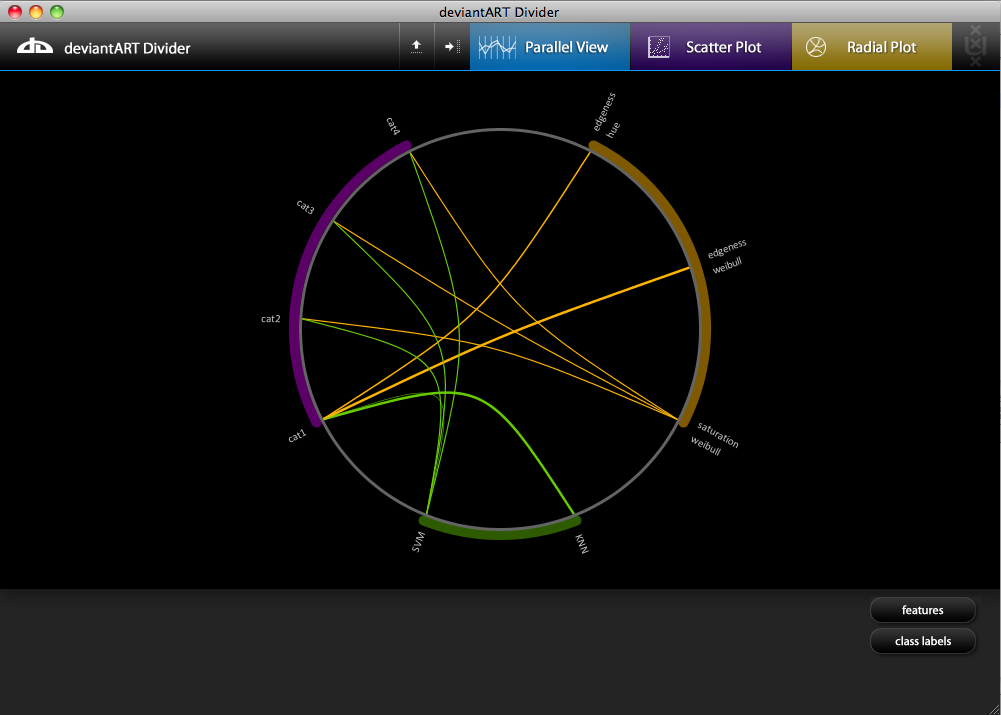
\includegraphics[width=1\linewidth]{img/visualization_radial.png}
  \caption{The visualization application displaying a radial plot that expresses the performance of the classification.}
  \label{fig:visualization_radial}
\end{figure}

Figure~\ref{fig:visualization_radial} shows the \textit{radial plot} visualization technique.
This visualization is not used to visualize the dataset, but to display the performance of the classification, e.g. how a certain feature performs on separating an artist from the other artists.
The circle is split into three regions (variables): artists or categories (purple), features (yellow), classifiers (green).
%Each of these regions represent a variable that plays an important role in the classification of images.
%Each variables consists of a limited number of values that were used during classification.
The thickness of a line between two nodes expresses the performance of the classification when both nodes are used together, i.e., thicker lines means better performance.
For example, a thick line between artist X and feature Y, means that feature Y is a good feature to separate artist X from the other artists.
